\documentclass[11point]{article}
% set the margins
\usepackage[left=25mm,right=25mm,top=20mm,bottom=20mm]{geometry}
% for displaying images
\usepackage{graphicx}
% for equation support, e.g. eqref
\usepackage{amsmath}
% for table support, e.g. toprule
\usepackage{booktabs}
% for multiple authors as a block
\usepackage{authblk}
% Custom enumerate item markers
\usepackage[shortlabels]{enumitem}
% for tables position
\usepackage{float}
% For in-text links
\usepackage{hyperref}

\newcommand{\note}[1]{\textbf{#1}}

\begin{document}

\title{INST0060 Investigation report:\\Hospital Queuing problem}
\author[*]{Group T1}
%\author{Auguste Baum}
%\affil[*]{Dept. of Information Studies}
%\affil[**]{Dept. of Physics \& Astronomy}
%\affil{Dept. of Natural Sciences}
\affil[ ]{University College London, WC1E 6BT}
%\affil[ ]{\textit {\{email1,email2\}@ucl.ac.uk}}
\date{\today}

\twocolumn[
\maketitle
]

\begin{abstract}
Queuing systems are a common subject of study in reinforcement learning. Here, we simulate a hospital with doctors and patients, each with their own characteristics, and use reinforcement learning to optimize the allocation of arriving patients to a queue.
\end{abstract}

\section{Introduction}
\label{sec:intro}

\subsection{Background}
In recent times, hospital queuing times have become a concern.
Because hospital represent clusters of vulnerable individuals, it can be of vital interest to limit the number of people standing in line or in a waiting room.

According to a 2015 study, on average Americans spent 84 minutes per visit in the hospital during the 2003-2010 period. \cite{Ray2015}
%In hospital situat are 61\% people spend 90-180 minutes in the queue of clinic before being seen by doctor, whereas 36.1\% patients spent less than 5 minutes with the doctor in the consulting room.\cite{Oche2013} Unorganized queues in hospital are always a depressing experience for us. Differing from standing in line for coffee, queuing in hospital makes people stressful and their health is at risk.

A long-term goal to accommodate the increasingly large flow of patients would be to improve healthcare infrastructures.
Yet, because staffing and finance issues are so context-sensitive in many countries, it is not possible to directly ascertain which strategy to follow.
However, a more efficient allocation of pre-existing resources can be beneficial in many cases.
%Here are some good advice to manage the queues: using internal labelling to simplify the triaging process, arranging emergency cases over anything else and making some records to further improve patient information management.\cite{Kirill2017}
Furthermore, some decisions in such complex systems could potentially be automated for higher reactivity and better performance.

Reinforcement learning is a form of goal-directed learning with interaction;
an agent learns how to respond to situations with certain actions so as to maximize a reward.
\cite{sutton2018reinforcement}
In a sense, a reinforcement learning agent explores and exploits past experience.

Queuing problems have been optimised using reinforcement learning in the past (such as traffic intersections \cite{soh2007modelling}), and hospitals have been modelled statistically as well. \cite{feng2018steady,Hagen2013}
%For instance, Markov decision control was applied on a simulated traffic intersection (modelled as an M/M/1 queue) to minimize queue length and waiting time.

%Feng and Shi studied hospital inpatient flow management as a discrete-time queuing system.
%They identified an approximation to the steady-state distribution of the number of jobs in the system, and proved that their approximation performs better than those based on constant-time coefficients when the number of servers is small in a single hospital.
%Their research provide us good suggestions on how to describe the patients flow at hospital as discrete‐time process. \cite{feng2018steady}

%There is another research explored some different queue models in intensive care units (ICU) and its influence on waiting time to severe case patients. 
%This report built a system-based simulation model to analyse the patient flow before entering ICU.
%This report divided all the patients into 9 different classes that are categorized by severity of patients and length of waiting time in queue.
%Similarly, our research classified doctors of different types related to their abilities and patients of their priority based on their severity. \cite{Hagen2013}



In this work, we use reinforcement learning to allocate patients to queues as efficiently as possible.
First, we will describe the system as modelled (with simplifying assumptions) and the methods used to learn policies.
Then, we will analyse the resulting policies in simple cases, to gauge the ability of learners compared to systematic or random policies and to human intuition.
We will also reflect on our experience of the project, discussing the various difficulties encountered and what steps were taken in response.

%\section{Background}
\section{Methods}

In the first instance, we tried modelling the hospital system as a Markov decision process (or MDP) in continuous time, in order to maintain proximity with both a real hospital system and the material we took away from the INST0060 lectures.
However, we quickly realised that we were not equipped to simulate a system in continuous time,
and that the complexity of the system (even with our simplifying assumptions) prevented us from using an MDP or table-lookup approach.
Hence, we decided to approximate a hospital system by a discrete-time process with a patient arrival every timestep and developed featurisations that allowed for the use of function approximation.

\subsection{Model characteristics}
The hospital contains servers (doctors) of different types, which correspond to their abilities.
Similarly, jobs (patients) have different priorities that warrant different services.
For example, a doctor of type 1 can treat a patient with priority 1 or lower, but a doctor of type 0 \emph{cannot} treat a patient with priority 1 or higher.

In general, if the highest doctor type is $N$ at initialisation, then it is expected that there be at least one doctor of each type $n\in \{0,1,\ldots,N\}$.
Each \emph{type of} doctor has an associated queue, hence thereafter we call ``queue $n$'' the unique queue which doctors of type $n$ draw from.
Newly arrived patients have needs sampled from $\{0,1,\ldots,N\}$ according to a known distribution and are allocated to a given queue in $\mathcal{A}=\{0,1,\ldots,N\}$ by an agent following a policy $\pi$.
Note that, once allocated, a patient may not change queues, though they \emph{may be allocated to a doctor who cannot treat them} (see Fig. \ref{fig:hospital_diagram}).
Once they are received by a doctor, if there is a discrepancy, the patient is sent away.

The state space is considered discrete, for simplicity. At each time step:
\begin{itemize}[nosep]
    \item a new patient arrives, with priority level sampled at random; 
    \item one or more doctors might be finished treating a patient; when that is the case, the ``cured'' patient leaves and is replaced by the next-in-line. 
\end{itemize}

Each individual doctor has their own efficiency, which is modelled by the probability of being done with a patient at each timestep.

Hence, if a skilled doctor happens to also be very fast, it might be beneficial to allocate low priority patients to their queue, to deplete the size of queues more quickly;
however, this runs the risk of making patients with high priority wait longer.

In this study, we restrict ourselves one doctor per type, as this still offers ample flexibility. The general case could be the subject of future work.
Similarly, though this study started with one queue \emph{per doctor} rather than per \emph{type} of doctor, we simplified the system after discussions with the module administrators and TAs.

\begin{figure}
    \centering
    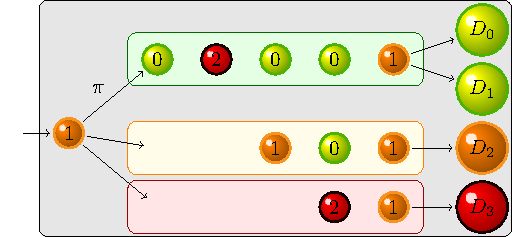
\includegraphics[width=0.9\columnwidth]{figures/hospital.pdf}
    \caption{A hospital with 4 doctors: two of type 0 ($D_0$ and $D_1$, green), one of type 1 ($D_2$, orange) and one of type 2 ($D_3$, red). A newly arrived patient with priority 1 is being allocated to a queue according to policy $\pi$.
    Note the priority 2 patient mistakenly sent to queue 0; they will not be sent away until they have reached the end of the queue.}
    \label{fig:hospital_diagram}
\end{figure}

One of the challenges associated with learning a policy to set balanced priorities between curing patients and keeping the hospital from getting too full.
Because of the behaviour of misallocated patients (see Fig. \ref{fig:hospital_diagram}), it can be more efficient for the agent to just misallocate patients from the start so as to keep the hospital empty.

The agent's actions tend to have very delayed consequences, which makes it difficult for it to link rewards and policy.
Further, originally the penalty for misallocation was set to trigger only when patients reached the doctor.
This mechanic was modified midway through the project to investigate its effect, and this will be the subject of Experiment 3.

\subsection{Learning}
Two well-known algorithms of RL are the Q-learning (QL) and the SARSA algorithms. \cite{sutton2018reinforcement}
SARSA is an on-policy algorithm,
meaning the agent learns the value of the state-action pair on the basis of the performed action.
By contrast, QL is an off-policy algorithm, where the state-action-value function (or \textit{q}-function) is estimated based on a greedy policy, which is not necessarily the currently implemented policy.
Generally, SARSA tends to exhibit faster convergence, while the performance of Q-learned policies tend to be higher. 
However, in SARSA the learner can easily get stuck in local minima, and QL tends to take longer to converge.

\subsection{Featurisation}

Even with the limited complexity of its modelling, the number of individual states in the hospital is extremely large, since each state includes the number of people in each queue, but also the types of patients and their waiting times.
In fact, it is countably infinite if the hospital occupancy in not bounded (which it is during training), so that a simpler representation (a simple vector) must be used for the agent to learn efficiently.

While at the beginning a few real numbers were used (such as the average number of patients per queue), later on an effort was made to include more information (real numbers, but converted to discrete values) and finally, one-hot vectors.
This last attempt was the most successful and will be applied throughout this work; the impact of featurisations will be the subject of experiment 1.

In this work, the systems of interest will be:
\setlist{left=0pt}
% Could use description environment
% I want to text to wrap all the way back because it's a waste of space
% Considering just breaking line after "Experiment:"
\begin{enumerate}[\bfseries {Experiment} 1:, wide, labelwidth=!, labelindent=0pt]
    %\DrawEnumitemLabel
    \item Two doctors (one of type 0 and one of type 1) with one featurisation and one learning algorithm. The 
    \item
    We analyse the behaviour of the agent as the frequency of urgent patients increases.
\end{enumerate}{}

%Featurisation in machine learning is the procedure of processing data to create features that makes machine learning algorithms work. If featurisation is built correctly, it increases the accuracy of prediction in machine learning algorithms by raw data processing. 

%In the simple example of Markov Decision Process of Stair Climbing, there are only two actions: climbing upstairs and going downstairs. Value function assigns values to states, and after definite updates, the value function in this model will remain unchanged values. The matrix of states in the stair climbing example also have fixed rows and columns, in which columns are the number of stairs and rows represents the values functions. 

%However, in our model of queueing problem in hospital, the states can be consider as infinite number. The patients are assigned to different queues, which correspond to their severity of illness. Similarly, the doctors have different types based on their abilities. Moreover, in each queue there could be a different amount of patients with different severities and wait times. To capture all the information, we could set the models as a limit of 30 people per queue, wait time of 40 time steps and 6 types of doctors totally. In this case, we could have more than $(30\times40\times3)^3 \approx 4\cdot10^{10}$ states. It is impossible to learn infinite number of states in our model. As a result, featurisation makes a great difference here to simplify our model with limited states. 
%Here are the basic steps of applying featurisation.
%\begin{enumerate}
%    \item Brainstorm on the classification of data and features.
%    \item Create features and set range of classification. 
%    \item Check the efficiency of feature the how good it works on model.
%    \item Start again from beginning until the features work perfectly.
%\end{enumerate}

%To discover a good final policy, six featurisations of our hospital model have been designed as follows.

%All featurisations include the average number of patients waiting in the different queues. Both Featurisation 1 and 2 use different thresholds to compare whether a given queue has more or fewer patients with a certain need. F1 compares the number of needy patients with thresholds 1 and 3 respectively and results in four conditions: no patients, one patient, patient number between 1 and 3, patients more than 3 and corresponsively update the list by 0, 1, 2, and 3. F2 updates the list every time when the patient number is not smaller than 2. 

%For F3, other than the first element, the following elements in the list represent the number of different patients with needs in each queue only and it adds total number of different patients in separate queues. F4 includes an additional element of the waiting time based on F3. For F5, the first element in the list is the need of the newly arrived patient, followed by the total number of patients in all the queues, the average need and waiting time in each queue.



%\subsection{Learning Algorithm}
%For the learning agent in Reinforcement Learning algorithm, there are two types of policy:
%\begin{itemize}
%    \item On-Policy: The learning agent learns the value function according to the current action derived from the policy currently.\cite{sutton2018reinforcement}
%    \item Off-Policy: The learning agent learns the value function according to the action derived from another policy.\cite{sutton2018reinforcement}
%\end{itemize}
%Sarsa (State-Action-Reward-State-Action) algorithm is an on-policy algorithm, which follows the policy it is evaluating. It uses the action performed by the current policy to learn the Q-value.
%Q-learning algorithm is slightly different from SARSA. Q-learning technique is an off-policy technique and uses the greedy approach to learning the Q-value.
%
%\subsubsection{Sarsa}
%Equation of Sarsa can be described as:
%\[
%\hat{q}(s_t,a_t)
%\leftarrow
%\hat{q}(s_t,a_t) +
%\alpha\left[
%    r_{t+1} +
%    \gamma\hat{q}(s_{t+1},a_{t+1}) -
%    \hat{q}(s_t,a_t)
%\right]
%\]
%As with Monte-Carlo, Sarsa learning can perform on-policy optimisation with temporal difference estimates using Q-estimates. The equations present the current state($s_t$), current action($a_t$), reward obtained ($r_{t+1}$), next state ($s_{t+1}$) and next action ($a_{t+1}$). This observation ($s_t$, $a_t$, $r_{t+1}$, $s_{t+1}$,  $a_{t+1}$) stands for the name of Sarsa: State Action Reward State Action. In our example of queue problem in hospital, current state represents the status of the patients in the queue and actions for patients are their choices to joining which doctor's queue according on their severity of illness.\\
%Our process of codes can be described as following seven steps:\\
%1. Import the required libraries and build the environment\\
%2. Define utility function (Sarsa) in learning process\\
%3. Initialize parameters of this function\\
%4. Training the learning agent\\
%5. Application of policies\\
%6. Evaluate the performance\\
%7. Visualisation of result
%\subsubsection{Q-Learning}
%Q-learning is an off-policy algorithm for TD learning. It learns the optimal policy even when actions are selected based on a more exploratory or even random policy. Its equation can be introduced as:
%
%\[\hat{q}(s_t,a_t)\leftarrow \hat{q}(s_t,a_t) + \alpha\left[r_{t+1}+\gamma \max_{a}\hat{q}(s_{t+1},a)-\hat{q}(s_t,a_t)\right] \]
%
%In which, $s$(state) and $a$(action) has the same definition as Sarsa's equation. $\alpha$  presents the the step length taken to update the estimation of q value. $\gamma$ is a discount factor for future rewards with range from $0$ to $1$. $r_{t+1}$ is the reward observed response to current action.



\section{Results}

\subsection{Experiment 1: Featurisations}

Here we demonstrate how the importance of the choice of feature vector.
The feature vectors below generally fall into two categories: one-hot vectors (featurisations 7-12) and non-one-hot vectors (featurisations 1-6).
These can be found in the \texttt{learning.py} file.
EXPLAIN EXPERIMENTAL CONDITIONS: which reward system, how many tests for each featurisation, which learning algo... try to justify choices

The data shown in \autoref{tbl:feat} implies that one-hot vectors are clearly the better choice since most of them achieve close to maximum reward. The upper bound of the reward in these simulations is 10 000. However, the difference between individual one-hot featurisations can also be significant.

Feature 12 appears to be the clear winner.It does not only achieve a higher reward on average but is also more consistent (given the lower deviation).The information that it takes into account is the level of sickness of the next patient to be allocated, the wait time for the first patient on each queue and the number of patients by types in each queue.

Mb should add a picture of the histogram of the allocated patients? reward evolution ?
Adding/removing some parameters in the table ?



The table below presents useful statistics about some of the featurisations.Each experiment is conducted 
100 times in order to obtain this data.
\begin{table}[H]
    \centering 
    \begin{tabular}{|l|l|l|l|}
    \hline
    Rewards & Mean & Median & Std.dev \\
    \hline
     feature 12 & 9260 & 9478 & 647 \\
    \hline
    feature 7 & 9041 & 9357 & 1247 \\
    \hline
    feature 8 & 8698 & 9141 & 1362 \\
    \hline
    feature 9 & 9067 & 9485 & 1072 \\
    \hline
    feature 10 & 941 & 1636 & 2540 \\
    \hline
    feature 11 & 8876 & 9523 & 1532 \\
    \hline
    feature 1 & 6953 & 7182 & 1271 \\
    \hline 
    \end{tabular}
    \caption{Rewards depending on the featurisation}
    \label{tbl:feat}
\end{table}

\subsection{Experiment 2: Model behaviour (code in \texttt{fastdoc\_exp.py})}
 In this experiment, we try	to characterise the behaviour of the agent in ambiguous situations.
The hospital has four doctors, of types 0 through 3. Doctor 3 (the most highly skilled) is also very efficient, while lower skilled doctors are equally slow.

\note{TBD}
We set the featurisation to \texttt{feature\_12}, the learning algorithm to SARSA and a reward system to penalise misallocations early and not penalise when occupancy is reached, as these seem to yield better performance overall.

Then, we gradually increase the frequency of type 3 patients.
When there are few, the agent should allocate many low priority patients to doctor 3 because it treats more quickly. However, when there are many, allocating low-priority patients to doctor 3 causes type 3 patients to wait longer, so we expect a decrease in total allocations to queue 3.

The results are shown in \autoref{fig:fast_doc}

\begin{figure}
    \centering
    % \includegraphics{figures/???}
    \caption{Behaviour of agent as priorities change. For each probability, the agent was trained for ??? episodes with ??? steps each.}
    \label{fig:fast_doc}
\end{figure}

\section{Discussion}

\section{Conclusion}


\section*{Declaration}
This document represents the group report submission from the named authors for the project assignment of module: Foundations of Machine Learning and Data Science (INST0060), 2019-20. In submitting this document, the authors certify that all submissions for this project are a fair representation of their own work and satisfy the UCL regulations on  plagiarism.

% to put references in
\bibliography{report}
% define the bibliography style
\bibliographystyle{plain}

\end{document}
